% !TEX TS-program = pdflatex
% !TEX encoding = UTF-8 Unicode

% Copyright (c) 2012, Edd Barrett <vext01@gmail.com>
% 
% Permission to use, copy, modify, and/or distribute this software for any
% purpose with or without fee is hereby granted, provided that the above
% copyright notice and this permission notice appear in all copies.
% 
% THE SOFTWARE IS PROVIDED "AS IS" AND THE AUTHOR DISCLAIMS ALL WARRANTIES
% WITH REGARD TO THIS SOFTWARE INCLUDING ALL IMPLIED WARRANTIES OF
% MERCHANTABILITY AND FITNESS. IN NO EVENT SHALL THE AUTHOR BE LIABLE FOR
% ANY SPECIAL, DIRECT, INDIRECT, OR CONSEQUENTIAL DAMAGES OR ANY DAMAGES
% WHATSOEVER RESULTING FROM LOSS OF USE, DATA OR PROFITS, WHETHER IN AN
% ACTION OF CONTRACT, NEGLIGENCE OR OTHER TORTIOUS ACTION, ARISING OUT OF
% OR IN CONNECTION WITH THE USE OR PERFORMANCE OF THIS SOFTWARE.

\documentclass{beamer}

%\usetheme{AnnArbor}
\usecolortheme{default}
\usecolortheme{orchid}
\usecolortheme{whale}
%\usecolortheme{seagull}
%\usepackage{serif}
\usepackage{bytefield}
\usepackage{listings}
\usepackage{alltt}
\usepackage{ulem}
\usefonttheme{professionalfonts}


 \usebackgroundtemplate{
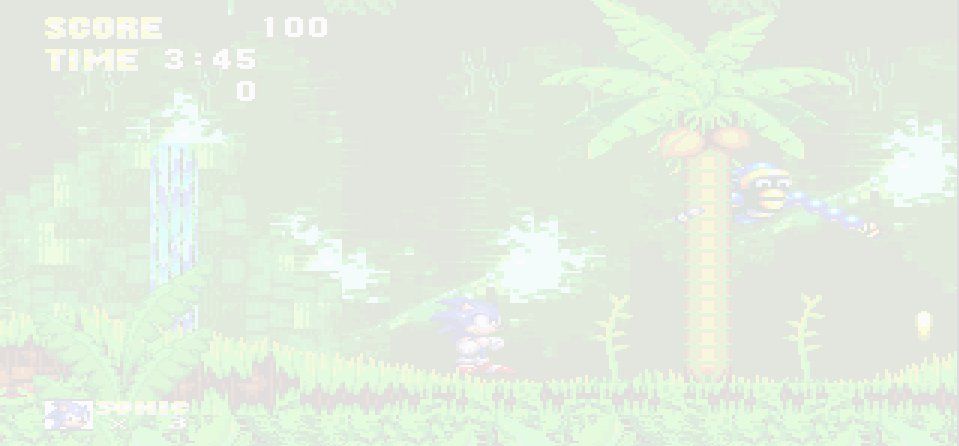
\includegraphics[width=\paperwidth,
height=\paperheight]{img/bg.jpg}
}

\title{Reversing Engineering SEGA Megadrive Games}
\author{Edd Barrett}
\date{\today}

\lstset{
  basicstyle=\ttfamily\small,
  breaklines=true,
  stringstyle=\ttfamily,
  framexleftmargin=1pt,
  backgroundcolor=\color{white}
}

\begin{document}

% ------------------------------

\begin{frame}[fragile]
  \titlepage
  \vspace{-4em}
  \begin{center}
  Twitter: @vext01
  \end{center}
\end{frame}

% ------------------------------

\AtBeginSection[]{%
  \begin{frame}<beamer>
  	\frametitle{}
  	\begin{block}{\inserttitle}
       \vspace{.5 em}
	{\huge \insertsection}
	\end{block}
    %\tableofcontents[sectionstyle=show/hide,subsectionstyle=hide/show/hide]
  \end{frame}
  \addtocounter{framenumber}{-1}% If you don't want them to affect the slide number
}
\section{Introduction}

\subsection{Why?}

\begin{frame}[fragile]


\frametitle{\insertsubsection}

\begin{itemize} 
\item When I was a kid I had a SEGA Megadrive (didn't we all).
\vfill
\item Since then I have learned a lot about reverse engineering.
\vfill
\item Curiosity led me to look at how these systems work.
\end{itemize}

\end{frame}

% ------------------------------

\subsection{Starting Out}
\begin{frame}[fragile]
\frametitle{\insertsubsection}

\vfill
I find the best way to learn about something is to have a clear goal.


\begin{block}{Goal 1}
\begin{center}
Sonic 3 -- Reverse the save game mechanism.
\end{center}
\end{block}

\vfill
And if I succeed:

\begin{block}{Goal 2}
\begin{center}
Make some tooling to help reverse other games too.
\end{center}
\end{block}
\end{frame}
\vfill

% ------------------------------

\section{SEGA Megadrive -- Overview}
\subsection{Basic Architcture}

\begin{frame}[fragile]
\frametitle{\insertsubsection}

A quick overview of the SEGA megadrive:

\begin{block}{CPU cores}
Basically a glorified m68k:

\begin{itemize}
\item Motorola m68000 -- 64K RAM, 7.61/7.67 MHz
\item Zilog Z80 -- 3.58 MHz
\end{itemize}
\end{block}

\vfill

\begin{block}{The rest}
\begin{itemize}
\item Yamaha YM2612 FM (Main sound chip)
\item Texas Instruments SN76489 PSG (Sq. Wave / White noise)
\item Custom graphics chip (VDP)
\end{itemize}
\end{block}

\end{frame}

% --------------------

\subsection{Game Cartridges}

\begin{frame}[fragile]
\frametitle{\insertsubsection}

\begin{center}
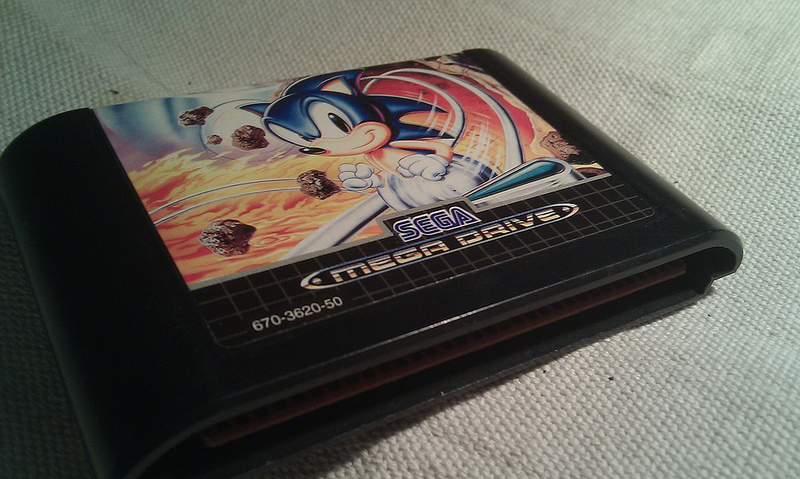
\includegraphics[height=0.7\textheight]{img/cart.jpg}
\end{center}

\end{frame}


\begin{frame}[fragile]
\frametitle{\insertsubsection}

\begin{center}
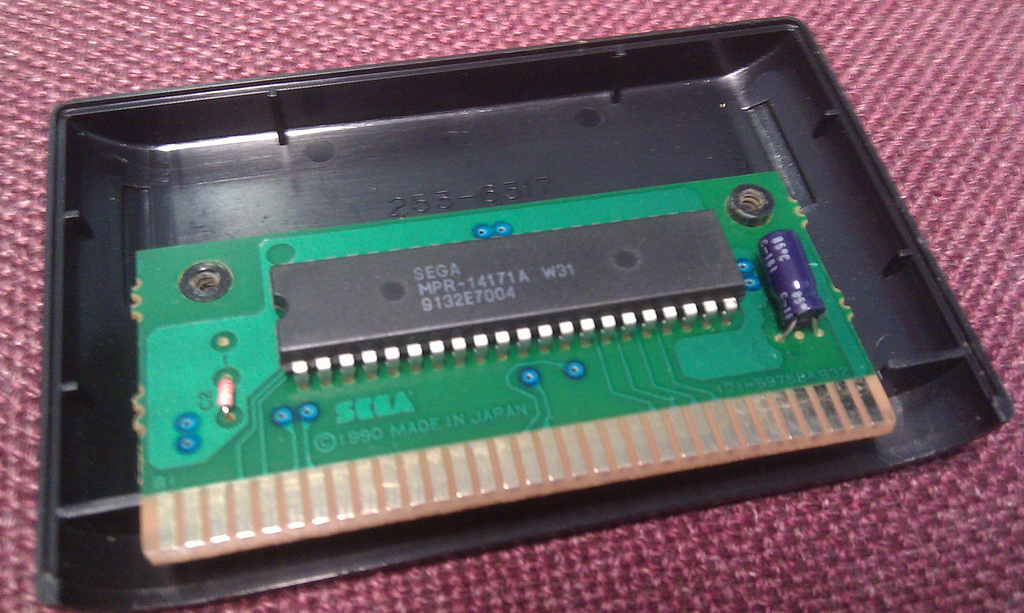
\includegraphics[height=0.7\textheight]{img/inside_cart.jpg}
\end{center}

\end{frame}

% ---

\begin{frame}[fragile]

\frametitle{\insertsubsection}

\begin{block}{Inside a Typical Cart}
\begin{itemize}
\item ROM
\begin{itemize}
\item Game instructions
\item Sprites
\item Music
\end{itemize}
\vfill

\item Save RAM (Optional)
\begin{itemize}
\item Stores persistent state. High scores, saves etc.
\item Usually a lithium cell retain memory
\end{itemize}
\vfill

\item Additional graphics hardware (Optional)
\begin{itemize}
\item For any ``special'' graphics capabilities
\item Eg. Sega Virtua Processor
\end{itemize}
\end{itemize}
\end{block}

\end{frame}

% ------------------------------

\subsection{Memory Map of the Megadrive}

\begin{frame}[fragile]
\frametitle{\insertsubsection}

\begin{center}
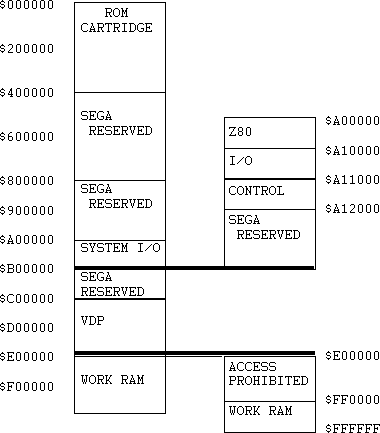
\includegraphics[height=.7\textheight]{img/mmap.png}
{~~~~\raggedright \footnote{Image borrowed from Nemesis}}
\end{center}

\begin{itemize}
\item {\small Thanks to the leaked sega2.doc we know about the memory layout}
\end{itemize}

\end{frame}

% ------------------------------

\subsection{Memory Map of a Game Cart}

\begin{frame}[fragile]
\frametitle{\insertsubsection}

\begin{itemize}
\item First 512 bytes are the ``cart header''.
\item The layout of the rest of the cart is specified inside the header.

\vfill

\begin{lstlisting}[basicstyle={\tt\tiny}]
% ./dgm_hdump ~/roms/Sonic\ the\ Hedgehog\ 3.bin 
Console Name : [SEGA GENESIS    ]
Copyright    : [(C)SEGA 1993.NOV]
Domestic Name: [SONIC THE             HEDGEHOG 3                ]
Overseas Name: [SONIC THE             HEDGEHOG 3                ]
Game Type    : [GM]
Product Code : [ MK-1079 -00]
Checksum     : a8 f2 
IO Support   : [J       ]
ROM Start    : 00 00 00 00 
ROM End      : 00 1f ff ff 
RAM          : 00 ff 00 00 00 ff ff ff 52 41 f8 20 00 20 00 01 00 20 03 ff 
RAM Present? : [RA]
RAM Start    : 0x200001
RAM End      : 0x2003ff
Modem Data   : [            ]
Memo         : [       ?ÿÿ  ÿ         ]
Release Country: []
\end{lstlisting}

\end{itemize}

\end{frame}

% ------------------------------

\section{Reversing the Sonic 3 Save RAM}

\subsection{How Do We Start -- The Electronic Engineer's Approach}

\begin{frame}[fragile]
\frametitle{\insertsubsection}

\begin{itemize}
\item Interface with Sonic 3 cart.
\item Dump save ram to disk somehow.
\item Identify field storing the level number in the save RAM.
\item Modify this field.
\item Upload modified RAM to cart.
\item Game on!
\end{itemize}

\vfill

Pretty difficult and probably requires extra hardware.

\end{frame}

% ------

\subsection{How Do We Start -- The Software Engineer's Approach}
\begin{frame}[fragile]
\frametitle{\insertsubsection}

Instead:

\begin{itemize}
\item Use emulator supporting save RAM emulation (Dgen).
\item Examine on-disk save RAM dump.
\item Identify field storing the level number in the save RAM.
\item Modify save directly on disk.
\item Game on!
\end{itemize}

\vfill

Requires no special hardware or electronics knowledge :)

\end{frame}

%--------------------------------

\subsection{Bindiffing Save RAM}

\begin{frame}[fragile]
\frametitle{\insertsubsection}

\begin{itemize}
\item First we need to find the ``interesting'' parts of save RAM.
\item We can use a bindiff tool find these.
\end{itemize}

\vfill

\begin{block}{Sonic 3 Example}
\begin{itemize}
\item In emulator, start game as Sonic -- Dump save RAM
\item Now start game as Tails -- Dump save RAM
\item Bindiff the two
\end{itemize}
\end{block}

\end{frame}

%--------------------------------

\begin{frame}[fragile]
\frametitle{\insertsubsection}

\begin{itemize}
\item I used \texttt{radiff2} from Radare2.
\begin{itemize}
\item \url{http://radare.org/y/}
\end{itemize}
\end{itemize}

\vfill

\begin{block}{Begin game with Sonic vs. Begin game with tails}

\begin{alltt}
0x0000016c 01 => 02		
0x000001cc 70 => c7		
0x000001ce 4f => fd		

0x000001f8 01 => 02     
0x00000258 70 => c7		
0x0000025a 4f => fd		
\end{alltt}
\end{block}

\vfill

\end{frame}


%--------------------------------

\begin{frame}[fragile]
\frametitle{\insertsubsection}

\begin{itemize}
\item I used \texttt{radiff2} from Radare2.
\begin{itemize}
\item \url{http://radare.org/y/}
\end{itemize}
\end{itemize}

\vfill

\begin{block}{Begin game with Sonic vs. Begin game with tails}

\begin{alltt}
0x0000016c 01 => 02		  <--- Looks like character field
0x000001cc 70 => c7		  <--- ?
0x000001ce 4f => fd		  <--- ?

0x000001f8 01 => 02		  <--- Same as above
0x00000258 70 => c7		  <--- just at different offset.
0x0000025a 4f => fd		  <--- For redundancy?
\end{alltt}
\end{block}

\vfill

\end{frame}

%--------------------------------

\begin{frame}[fragile]
\frametitle{\insertsubsection}

\begin{itemize}
\item Tried changing the character field
\item Either 0x0 or 0x3 is likely to be Sonic+Tails
\item Cart resets save RAM.
\item In all likelihood the unknown bytes are a checksum.
\end{itemize}

\vfill

\begin{center}
{\Huge ?}
\end{center}

\pause

\vfill

\begin{itemize}
\item Asked for help on ASSEMbler Games forum.
\begin{itemize}
\item \url{http://www.assemblergames.com/forums/}
\end{itemize}
\end{itemize}

\vfill

\end{frame}

%--------------------------------

\subsection{A Response}

\begin{frame}[fragile]
\frametitle{\insertsubsection}

Someone called ``Jorge Nuno'' replied to my post:
\vfill


\begin{lstlisting}[basicstyle={\tt\scriptsize}]
For the "checksum" this was from an old conversation between
me and him [Tmee]:

---8<---
OK Save Ram it is copied into 0xFFFFE600. And I think this
is the code that verifies the magic checksum:

sub_C362:
    moveq #0,d7
loc_C364:
    move.w (a6)+,d5
    eor.w d5,d7
    lsr.w #1,d7
    bcc.s loc_C370
    eori.w #$8810,d7
loc_C370:
    dbf d6,loc_C364
    rts

Need to checkout a6...
Probably d7 contains the result. 
---8<---
\end{lstlisting}

\end{frame}

% -----

\begin{frame}[fragile]
\frametitle{\insertsubsection}

\texttt{Oh, and\ldots}
\vfill\pause

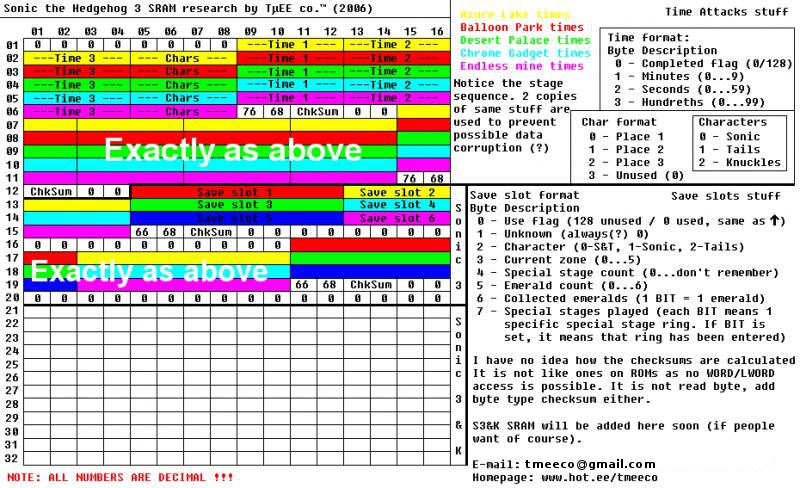
\includegraphics[width=\textwidth]{img/S3SRAM.jpg}

\end{frame}

%--------------------------------

\subsection{dgm\_s3ramgen}

\begin{frame}[fragile]
\frametitle{\insertsubsection}

\begin{itemize}
\item Mex and I reimplemented the checksum in C.
\item Wrote a tool to generate custom save RAMs for Sonic 3.
\end{itemize}

\begin{lstlisting}[basicstyle={\tt\scriptsize}]
Usage:  dgm_s3ramgen [options] outputfile

Options:
  -c num        Character select (0=ST, 1=S, 2=T)
  -e num        Emeralds (8-bitfield)
  -h            Show help
  -M            Make a MEGA-RAM (fully complete RAM)
  -p            Pad (word-align) RAM
  -s num        Choose slot to change
  -x num        Debug level (0-3)
  -z num        Choose zone (0-6)
\end{lstlisting}

\vfill

Eg. RAM with save slot 1 with S+T on zone 4 with 2 emeralds:\\{\tt dgm\_s3ramgen -s1 -c0 -z3 -e3 -p myramfile}


\end{frame}

% http://www.assemblergames.com/forums/showthread.php?37200-Reverse-Engineering-The-Save-Ram-on-A-Sonic-3-Genesis-Megadrive-Cartridge

\section{Goal 2: Tooling to Help}

\subsection{We Won't Always be So Lucky}

\begin{frame}[fragile]
\frametitle{\insertsubsection}


\vfill
\begin{itemize}
\item Now we know roughly what is involved in reversing save RAMs
\vfill
\item We won't be so lucky for every game.
\begin{itemize}
\item Ie. If I had not had a response on the forum, what would I do?
\end{itemize}
\vfill
\item I would have to have found checksum code myself.
\vfill
\item A tool which can help can be used to reverse other games.
\end{itemize}

\vfill

\end{frame}

% ----

\subsection{How to Find the Checksum Code in Sonic 3?}

\begin{frame}[fragile]
\frametitle{\insertsubsection}

\begin{itemize}
\item We need to know the PC (program counter) when the checksum is written. \textsc{Watchpoints}
\vfill
\item We need to be able to disassemble code we find here. \textsc{Disassembler}
\vfill
\item We need to read registers and memory to understand what code does. \textsc{Inspection}
\vfill
\item Perhaps we need to look at registers and memory \emph{just before} the checksum is generated. \textsc{Breakpoints}
\end{itemize}

\pause

\begin{center}
Looks like I am writing a debugger then\ldots
\end{center}

\end{frame}

% ----

\subsection{Implementing a Debugger}

\begin{frame}[fragile]
\frametitle{\insertsubsection}

\begin{itemize}
\item Take existing emulator and modify.
\item I chose Dgen/SDL
\end{itemize}

\vfill

\begin{block}{Dgen/SDL}
\begin{itemize}
\item Pretty good (fast) emulator
\item Open-source
\item Mature --  1999-2012 -- Dgen originally designed for DOS.
\item Cross platform -- well \ldots UNIX + windows
\item Original developers MIA -- Currently maintained by zamaz
\item Written in C++
\end{itemize}
\end{block}

\vfill

{\Large ``Dgen runs well on a P2-233''~~~~:P}

\end{frame}

\subsection{Implementing a Debugger}

\begin{frame}[fragile]
\frametitle{\insertsubsection}

\begin{itemize}
\item Take existing emulator and modify.
\item I chose Dgen/SDL
\end{itemize}

\vfill

\begin{block}{Dgen/SDL}
\begin{itemize}
\item Pretty good (fast) emulator
\item Open-source
\item Mature --  1999-2012 -- Dgen originally designed for DOS.
\item Cross platform -- well \ldots UNIX + windows
\item Original developers MIA -- Currently maintained by zamaz
\item Written in C++
\end{itemize}
\end{block}

\vfill

{\Large ``Dgen runs well on a P2-233''~~~~:P}

\end{frame}

\begin{frame}[fragile]
\frametitle{\insertsubsection}

\begin{itemize}
\item CPU cores pretty well written and made the task pretty easy.
\begin{itemize}
\item Musashi for m68k (from Mame project)
\item CZ80 for z80
\end{itemize}
\vfill
\item The only challenging aspect was to make the debugger \emph{fast}.
\end{itemize}

\vfill

\end{frame}

% ---

\subsection{Eg. Making Breakpoints \emph{Fast}}
\begin{frame}[fragile]
\frametitle{\insertsubsection}

\begin{lstlisting}
#define MAX_BREAKPOINTS                 64
struct dgen_bp debug_bp_m68k[MAX_BREAKPOINTS];
\end{lstlisting}

\vfill

\begin{itemize}
\item After each instr, we have to check if any of these BPs will fire
\item Checking 64 BPs if only 1 is used is wasteful (and slow)
\item Do as little work as possible by storing BPs cleverly.
\end{itemize}


\vfill


\begin{center}
\begin{bytefield}{32}
\begin{rightwordgroup}{BAD!}
   \bitbox{1}{*}
   \bitbox{1}{*}
   \bitbox{1}{}
   \bitbox{1}{*}
   \bitbox{1}{}
   \bitbox{1}{}
   \bitbox{1}{*}
   \bitbox{1}{*}
   \bitbox{1}{*}
   \bitbox{1}{}
   \bitbox{1}{*}
   \bitbox{4}{\ldots}
\end{rightwordgroup}
\end{bytefield}
\end{center}

\vfill

\begin{center}
\begin{bytefield}{32}
\begin{rightwordgroup}{Better}
   \bitbox{1}{*}
   \bitbox{1}{*}
   \bitbox{1}{*}
   \bitbox{1}{*}
   \bitbox{1}{*}
   \bitbox{1}{*}
   \bitbox{1}{*}
   \bitbox{1}{}
   \bitbox{1}{}
   \bitbox{1}{}
   \bitbox{1}{}
   \bitbox{4}{\ldots}
\end{rightwordgroup}
\end{bytefield}
\end{center}


\vfill

\end{frame}

% --------

\subsection{Eg. Making Breakpoints \emph{Fast} Again}
\begin{frame}[fragile]
\frametitle{\insertsubsection}


Another optimisation:
\vfill

\begin{block}{Too Slow}
\begin{enumerate}
\item Execute single instruction
\item Check if breakpoint fires
\item Draw screen
\item Goto 1
\end{enumerate}
\end{block}

\vfill

\begin{block}{Faster}
\begin{enumerate}
\item Register CPU step handler in Musashi core.
\item Execute as many instructions as possible (up to frame limit)
\begin{itemize}
\item CPU calls a handler after each instruction (last slide)
\item End current burst of instructions only if we need to break.
\end{itemize}
\item Draw screen
\item Goto 1
\end{enumerate}
\end{block}
\vfill

\end{frame}

\subsection{Demo}
\begin{frame}[fragile]
\frametitle{\insertsubsection}


{\huge A quick demo:}

\begin{itemize}
\item Insert watch point on the checksum bytes
\begin{itemize}
\item {\tt watch 0x002001cd 4}
\end{itemize}
\item From here we can find the checksum code
\end{itemize}

\end{frame}

\subsection{My Code is Free!}
\begin{frame}[fragile]
\frametitle{\insertsubsection}

\begin{block}{My ROM header dumper and Sonic 3 RAM gen tooling}
\url{https://github.com/vext01/dgmtools}
\end{block}

\vfill

\begin{block}{My Dgen/SDL Debugger}
Is included in Dgen/SDL as of version 1.30

\url{http://dgen.sourceforge.net/}
\end{block}

\end{frame}


\section{What is Next?}

\subsection{Future Distractions}

\begin{frame}[fragile]
\frametitle{\insertsubsection}

\begin{itemize}
\item Reverse some more games
\vfill
\item Implement Z80 watch and break points
\vfill
\item Fix dgen/SDL bugs
\vfill
\item Make some games for the Megadrive?
\begin{itemize}
\item In assembler or C
\end{itemize}
\end{itemize}

\end{frame}

% -----

\end{document}
